% last updated in April 2002 by Antje Endemann
% Based on CVPR 07 and LNCS, with modifications by DAF, AZ and elle, 2008 and AA, 2010, and CC, 2011; TT, 2014; AAS, 2016

\documentclass[runningheads]{llncs}

\usepackage{amsmath,amssymb} % define this before the line numbering.
\usepackage{ruler}
\usepackage{color}
\usepackage[width=122mm,left=12mm,paperwidth=146mm,height=193mm,top=12mm,paperheight=217mm]{geometry}

\usepackage{multirow}
\usepackage{graphicx}
\usepackage{subfig}
\usepackage{floatrow}
\captionsetup{labelsep=period}

\usepackage{booktabs}
\usepackage{standalone}

\usepackage{siunitx}


\usepackage[acronym]{glossaries}
\newacronym{acr::lod}{LoD}{Level of Detail}
\newacronym{acr::lidar}{LiDAR}{Light Detection And Ranging}
\newacronym{acr::dsm}{DSM}{Digital Surface Model}

\newcounter{SubFigCounter}
\setcounter{SubFigCounter}{1}

\begin{document}

\pagestyle{headings}
\mainmatter{}
\def\ECCV18SubNumber{***}  % Insert your submission number here

\title{Semantic Evaluation of 3D city models}

\titlerunning{ECCV-18 submission ID \ECCV18SubNumber}

\authorrunning{ECCV-18 submission ID \ECCV18SubNumber}

\author{Anonymous ECCV submission}
\institute{Paper ID \ECCV18SubNumber}

\maketitle

\begin{abstract}
    We are tackling the problem of 3D model reconstruction quality evaluation. Currently, no scalable approach has been proposed to semantically assess automatic reconstruction methods output. One must rely on the presence of high precision models that are not easily affordable. In our approach, we try to predict building models quality based on its geometry and available remote sensing data.
    \keywords{3D urban modeling, Quality assessment.}
\end{abstract}

\section{Introduction}

    3D urban models have a wide application range. They can be used for ludic purposes (video games or tourism) as much as they can be vital in more serious domains (for instance: run-off water and microclimate simulation or urban or security operations planification)~\cite{Biljecki2015},~\cite{Musialski2012}. Therefore, automatic urban reconstruction is the focus of both scientific research and industrial activity. However, the problem is still unresolved~\cite{Musialski2012},~\cite{rottensteiner2014results}. In fact, besides the seamless nature of reconstituted models, current algorithms are greedy in time, lack genericity --- regarding urban different possible urban scenes --- and produce a great deal of erroneous buildings. As such, human intervention is needed either in interaction within the reconstruction pipeline or as a post-processing clean-up step. The later being a long and tedious task~\cite{Musialski2012}, automatizing urban reconstruction evaluation can be helpful, especially in a production environement.\\

    This work focuses on evaluating polyhedral building models resulting from urban reconstruction methods. Polyhedral models are more compact than triangle meshes extracted from mutliview images or point clouds. In consequence, these models hold more semantic information as each facet corresponds to a fa\c{c}ade, a roof or any well defined morphological building face. In counterpart, they are less efficient when it comes to fidelity to input data. Thus, reconstruction algorithms try to find a good compromise between compacity and semantics on one hand, and fidelity on the other. Depending on the input data spatial resolution, the urban scene in question and the aimed application, the reconstruction result has a certain \acrfull{acr::lod}~\cite{kolbe2005citygml}. A \acrshort{acr::lod} $1$ model is a simple building extrusion. A \acrshort{acr::lod} $2$ model considers geometric simplification of buildings, ignoring superstructures, such as dormer windows and chimneys. These are taken into account in the next \acrshort{acr::lod} $3$. We will stick, from hereon, to these \acrshort{acr::lod} definitions as in~\cite{verdie2015lod}, since \glspl{acr::lod} are still subject to discussion~\cite{2016_ceus_improved_lod}.\\

     Finding a good reconstruction compromise involves answering some hard problems for which the solution is not guaranted to be found in polynomial time {\color{blue} (graph minimum cut~\cite{Taillandier2005},~\cite{Bredif2008} \dots)}. However, verifying these solutions could be answered much more easily. This motivates the need for a well suited quality assessement paradigm. Since the diagnosed models are well structured, an unrestricted evaluation based on data fidelity indices as in~\cite{berger2013benchmark}, is too general. It should also ignore format issues or geometric consistencies as studied in~\cite{ledoux2018val3dity}. In fact, these must be studied well before this stage. The semantic evaluation will only take into account building semantics through the detection and the categorization of modeling errors that can affect these buildings. The herein defined evaluation can, thus, be used for:
    \begin{itemize}
        \item \textbf{Building models correction}: automatically or interactively correct building models based on the detected errors;
        \item \textbf{Change detection}: where change can be considered as a modeling error or implicitly detected from other errors.
        \item \textbf{Reconstruction method selection}: based on the comparison of the designated algorithms performances on errors of interest;
        \item \textbf{Crowd-sourcing evaluation}: by categorizing user behaviors during crowd sourced modeling and vandalism detection.
    \end{itemize}

    \begin{figure}
        \begin{center}
            \includestandalone[mode=buildnew, width=\textwidth]{graphical_abstract}
            \caption{\label{fig::pipeline} The semantic evaluation paradigm proposal. }
        \end{center}
    \end{figure}

     3D urban reconstruction semantic evaluation has not been thouroughtly studied until now. Only one benchmark~\cite{rottensteiner2014results} exists but is not widely used for comparison~\cite{Lafarge2012},~\cite{nguatem2017modeling},~\cite{li2016boxfitting}. Usually reconstruction evaluation is based on visual inspection~\cite{Durupt2006},~\cite{MacayMoreia2013} or geometric precision indices~\cite{Kaartinen2005} without any localized semantic dimension. This work essentially proposes:
    \begin{itemize}
        \item a new \textbf{error taxonomy}, independent from any reconstruction approach or urban scene;
        \item the formulation of the evaluation problem as a \textbf{supervised classification} one that predicts previously defined errors that can affect the building model.
        \item a simple \textbf{baseline for features} is extracted from the model to feed a classifier for error prediction.
        \item {\color{blue} Adaptibility and flexibility of framework}.
    \end{itemize}

\section{Related Work}

Quality assessment methods can be classified based on two criteria: the type of their output or the reference data they use.
\subsubsection{Reference Data Types.}
All quality assessment methods need a reference data to be matched with. Indeed, existing approaches compare the 3D reconstructed building models to:
\begin{itemize}
    \item \textbf{Manually plotted ground truth} data with a higher spatial accuracy. These models can be obtained either through field measurements~\cite{Kaartinen2005},~\cite{Voegtle2003} with the highest possible precision ($\sigma(\text{error}) \approx \SI{0.05}{\meter}$), or using stereo-plotting~\cite{Kaartinen2005},~\cite{Zeng2014}. However this kind of data is not easily to come by.
    \item \textbf{Raw sensor data}. For instance, models can be compared to \acrfull{acr::lidar} point clouds~\cite{Akca2010},~\cite{Lafarge2012},~\cite{li2016boxfitting} or oriented aerial images~\cite{boudet2006supervised},~\cite{Michelin2013}. Although these are easier to get than the previous ones, they are low on structural and semantic informations for the sake of evaluation.
\end{itemize}
\subsubsection{Evaluation Output Types.}
The quality assessment methods can produce two kinds of outputs:
\begin{itemize}
    \item \textbf{Geometric fidelity indices}: they can summarize the quality of the whole assessed model. These indices are computed at different scales: points of interest (such as corners or edge points) average precision~\cite{Kaartinen2005},~\cite{Voegtle2003}, surface discrepancy~\cite{Kaartinen2005},~\cite{Henricsson1997},~\cite{Zeng2014},~\cite{Lafarge2012},~\cite{li2016boxfitting} or volume discrepancy to reference data~\cite{Zeng2014}. These outputs have the drawback of being too general for the special case of urban polyhedral models. In this case, far from surface reconstruction evaluation~\cite{berger2013benchmark}, we need to pinpoint specific types of errors that can be easily corrected once identified~\cite{OudeElberink2010}.
    \item \textbf{Semantic errors}: they identify topological and geometric errors that affect polyhedral models. One example of such taxonomy is the traffic light paradigm (correct acceptable, generalized and rejected)~\cite{boudet2006supervised}. However, these error depend on a vague definition of the ``generalized'' level. In addition, this taxonomy does not help to localize the model shortcomings. Another solution is to look at the issue at hand through the used reconstruction algorithm perspective. For instance, defects are arranged, in~\cite{Michelin2013}, into footprint errors (erroneous outline, inexistent building, missing inner court and imprecise footprint), intrinsic reconstruction errors (over segmentation, under segmentation, inexact roof and Z translation) and vegetation occlusion errors. In the later methods, the evaluation is the result of a supervised classification where predicted classes are defects listed in the taxonomy. Features are extracted from high spatial resolution (\SIrange{20}{25}{\cm}) oriented aerial images and \glspl{acr::dsm} by 3D segments and texture correlation scores comparison~\cite{boudet2006supervised},~\cite{Michelin2013}. In spite of the contribution with semantic information for quality evaluation, taxonomies can over-fit to a special urban scene or a reconstruction algorithm.
\end{itemize}

This work aims at devising a quality evaluation paradigm using no reference data, or, at least, the most available ones, that detects semantic localized errors independent from reconstruction methods and assessed models.

\section{Problem Formulation}

To evaluate reconstructed input models, an error taxonomy is established. Depending on the evaluation objectives, we deduce error labels that will be used to predict model defects. Buildings are thus annotated in order to train a supervised classifier model that will be used for prediction on other reconstituted models.\\

The error taxonomy is \textbf{agnostic} towards reconstructed inputs and \textbf{parameterizable}. This flexibility and independence means that, at runtime, the evaluation process does not involve heavy computing. Furthermore, it does not require any heavy reference data aside the annotated objects on which the classifier is pretrained.\\

The quality assessment pipeline is modular. Building models are represented by intrinsic geometric features extracted from the model facets graph. If available, the classifier can also be fed additional depth related features, based on the comparison of the model altimetry and the \acrshort{acr::dsm}, in case of aerial reconstruction, or, in general, any depth map comparison. Last but not least, radiometric information can be incorporated to the pipeline through aerial (orthogonal or oriented) or street view images.

\subsection{Error Taxonomy}
In order to build a generic and flexible taxonomy, we rely on two criteria for error compilation: the building \acrshort{acr::lod} and the error semantic level --- which is named henceforth \textit{finesse}. Each \textit{finesse} is associated to a natural integer starting from $0$. Errors with maximal \textit{finesse} are called \textit{atomic} errors. These last defects could be correlated, heuristically, to unit actions from an operator, or an algorithm, needed to correct the input model.

\subsubsection{A general layout.}
The main idea of hierarchization is to enable modularity in the taxonomy, and thus achieve a strong flexibility towards input urban scenes and desired error precision. A general layout is drawn herein before filling in the detailed error descriptions.\\

At a first level, model qualifiability is studied. In fact, aside from formatting issues or geometric inconsistencies~\cite{ledoux2018val3dity}, other reasons can render building models unqualifiable. For instance, buildings are occluded by vegetation. In general, input models can be impaired by some pathological cases that are outside our evaluation framework. In consequence, \textit{Qualifiable} models will be distinguished from \textit{Unqualifiable} buildings. This first qualification degree corresponds to the $\textit{finesse} = 0$.\\

At the next \textit{finesse} level ($\textit{finesse} = 1$), a qualifiable building reconstruction correctness is predicted. It is the lowest level of semantization at which the evaluation of a model is expressed. It is either \textit{Valid} or \textit{Erroneous}.\\

Model errors are to be grouped into three families depending on the underlying \acrshort{acr::lod}. The first family of errors (``\textit{Building Errors}'') affects the building in its entirety. It corresponds to an accuracy evaluation at $\acrshort{acr::lod}0\text{ } \cup \text{ }\acrshort{acr::lod}1$. At the next $\acrshort{acr::lod}2$, the family error assembles defects that can damage fa\c{c}ade or roof fidelity. The last error family, \textit{i.e.} ``\textit{Superstructure Errors}'', describes errors that involve superstructures modeled at $\acrshort{acr::lod}3$.\\

Each family contain atomic errors of maximal $\textit{finesse} = 3$. These errors are semantically independent, although they can co-occur in the same building model, in the same error family as much as across different ones. They represent particular topological or geometric defects. Topological errors translate structurally inaccurate modeling, while geometric ones pick up geometric positioning inaccuracies.\\

A scoring system can be attributed to this taxonomy. Each \textit{atomic} error will be attributed a score based on the quality assessment objective. This score, from \SIrange{0}{10}{}, describes the confidence level in the defect presence. At $10$ the error must be certainly detected, compared to $0$ where the error must surely not exist. Errors of lower \textit{finesse} inherit their score from their children. The presence of only one child error implicates the presence of its parent, at least, at the same level of confidence. Hence, the parent error category is attributed the maximum score of its children errors score.\\

At evaluation time, three parameters play a role in determining which error labels to consider. The first is the desired \textbf{\acrlong{acr::lod}}. Every reconstruction method targets a certain set of \glspl{acr::lod}. They cannot be evaluated at only one degree. In consequence, at a predefined \acrshort{acr::lod}, all error families involving higher order details will be ignored. Depending on the final use of qualification, a \textbf{finesse} level might be preferred. It is the second evaluation parameter, as errors are reported only at the appropriate semantic level. The last one is error \textbf{exclusivity}. This family error hierarchization is based on the modeling minuteness. If errors of a certain \acrshort{acr::lod} are detected, the more detailed ones are considered meaningless.

\subsubsection{Application diversity.}
Depending on the application of the reconstructed buildings, a set of errors can be judged irrelevant. For instance, for an urban planner that studies run-off water simulation, instantiating each building depending on its ownership might seem unnecessary. However a house insurer will be interested at knowing which building might be affected after a flood, in order to estimate the ensuing pecuniary loss. That is why the evaluation framework should be as open as much as final application diversity.\\

The presented taxonomy structure offers a great number of levers for that sake while being agnostic to these applications. Defects can be filtered out by fixing the previously defined parameters. It can also be refined by simply thresholding over them. A more subtle way of leveraging these scores is to ask the final user to reannotate model errors by attributing scores based on their model use. This can be done offline, but also in an active semi-supervized setting taking advantage of model precomputed similarities.\\

\subsubsection{The aerial reconstruction case.}
  \begin{figure}
        \begin{center}
            \includestandalone[mode=buildnew, width=\textwidth]{taxonomy_tree}
            \caption{\label{fig::pipeline} The proposed taxonomy illustration. }
        \end{center}
    \end{figure}
This study is, henceforth, narrowed to the aerial reconstruction case. The objective is to reconstruct large urban scenes using aerial oriented images and, if available, \acrshort{acr::lidar} point clouds. We will use these data  to confront with the modeled buildings.\\

In our case, we evaluate $2.5$D buildings. We propose these \textit{atomic} errors:
	\begin{itemize}
		\item \textbf{Building errors family}:
        \begin{itemize}
        	\item Under segmentation: two or more buildings are modeled as one;
            \item Over segmentation: one building is subdivided into two or more buildings;
            \item Inexact footprint: erroneous building footprint, where it groups geometric inaccuracies and topological defects as missing inner courts ($\equiv$ not the right number of polygon holes);
            \item Imprecise height: wrong building height estimation;
        \end{itemize}
		\item \textbf{Facet errors family}:
        \begin{itemize}
        	\item Under segmentation: two or more facets are modeled as one;
            \item Over segmentation: one facet is subdivided into two or more facets;
            \item Inexact segmentation: facet edges are inaccurate;
            \item Imprecise slope: wrongful facet slope estimation.
        \end{itemize}
	\end{itemize}

    \thisfloatsetup{heightadjust=object}
    \begin{figure}[H]
        \begin{center}
            \ffigbox{
                \ffigbox[\FBwidth]
                {
                    \begin{subfloatrow}[4]
                        \captionsetup{labelformat=brace, justification=raggedright}
                        \ffigbox[\FBwidth]{\caption{Under Segmentation.}\label{fig::under_bul}}{\fbox{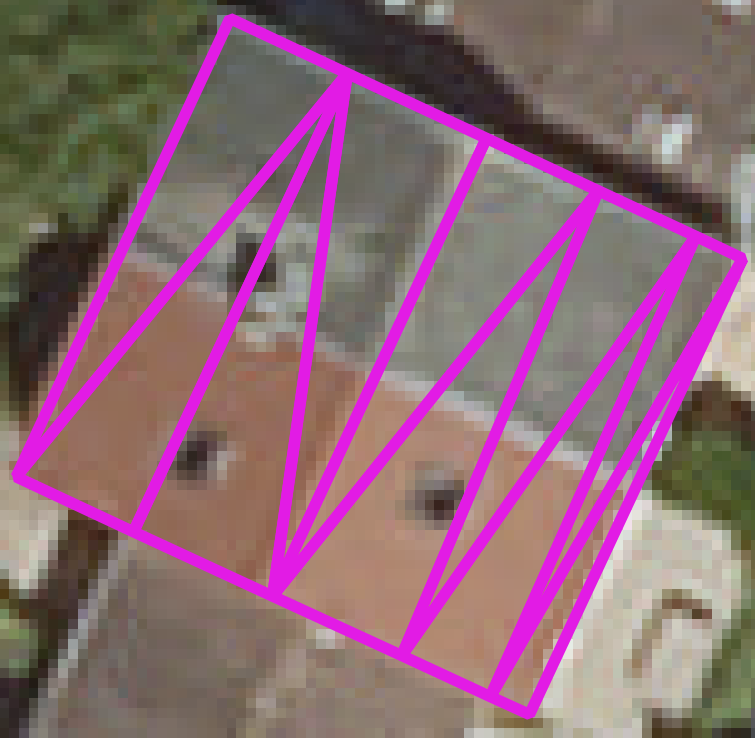
\includegraphics[width=.24\textwidth]{images/Building_Errors/under_segmentation}}}
                        \ffigbox[\FBwidth]{\caption{Over segmentation.}\label{fig::over_bul}}{\fbox{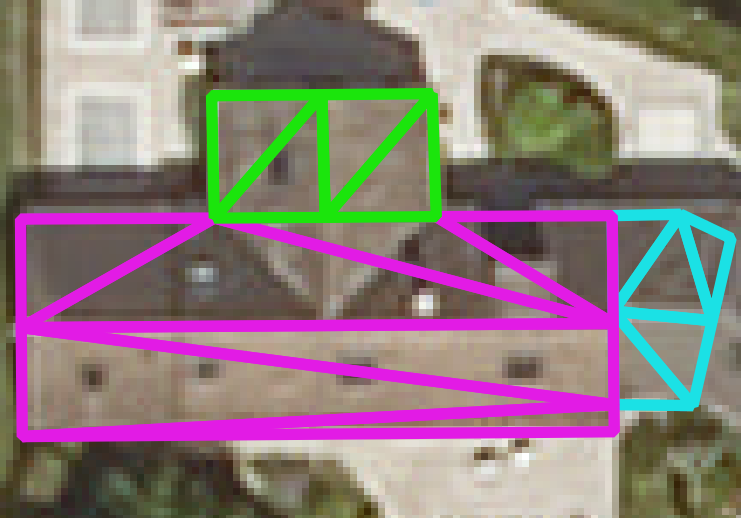
\includegraphics[width=.24\textwidth]{images/Building_Errors/over_segmentation}}}
                        \ffigbox[\FBwidth]{\caption{Inexact footprint.}\label{fig::footprint}}{\fbox{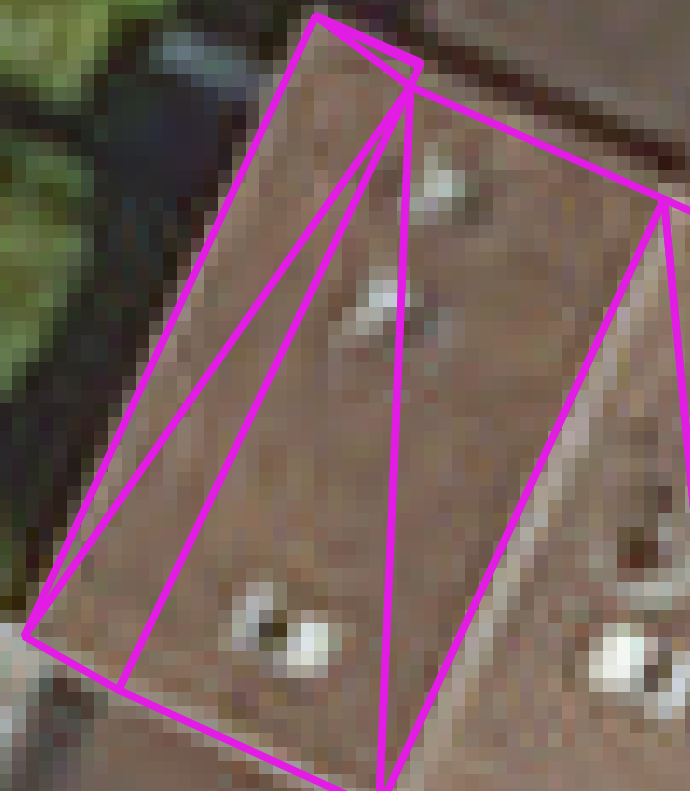
\includegraphics[width=.24\textwidth]{images/Building_Errors/footprint}}}
                        \ffigbox[\FBwidth]{\caption{Imprecise height.}\label{fig::too_low}}{\fbox{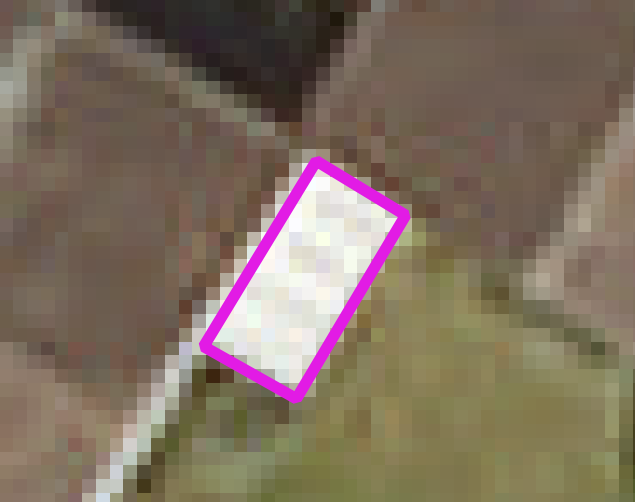
\includegraphics[width=.24\textwidth]{images/Building_Errors/altimetric}}}
                    \end{subfloatrow}
                }
                {
                    \renewcommand\figurename{}
                    \renewcommand{\thefigure}{(\roman{SubFigCounter})}

                    \caption{Building errors family samples.}\label{fig::bul_err}
                    \refstepcounter{SubFigCounter}
                }
                \ffigbox[\FBwidth]
                {
                    \begin{subfloatrow}[4]
                        \captionsetup{labelformat=brace, justification=raggedright}
                        \ffigbox[\FBwidth]{\caption{Under Segmentation.}\label{fig::under_fac}}{\fbox{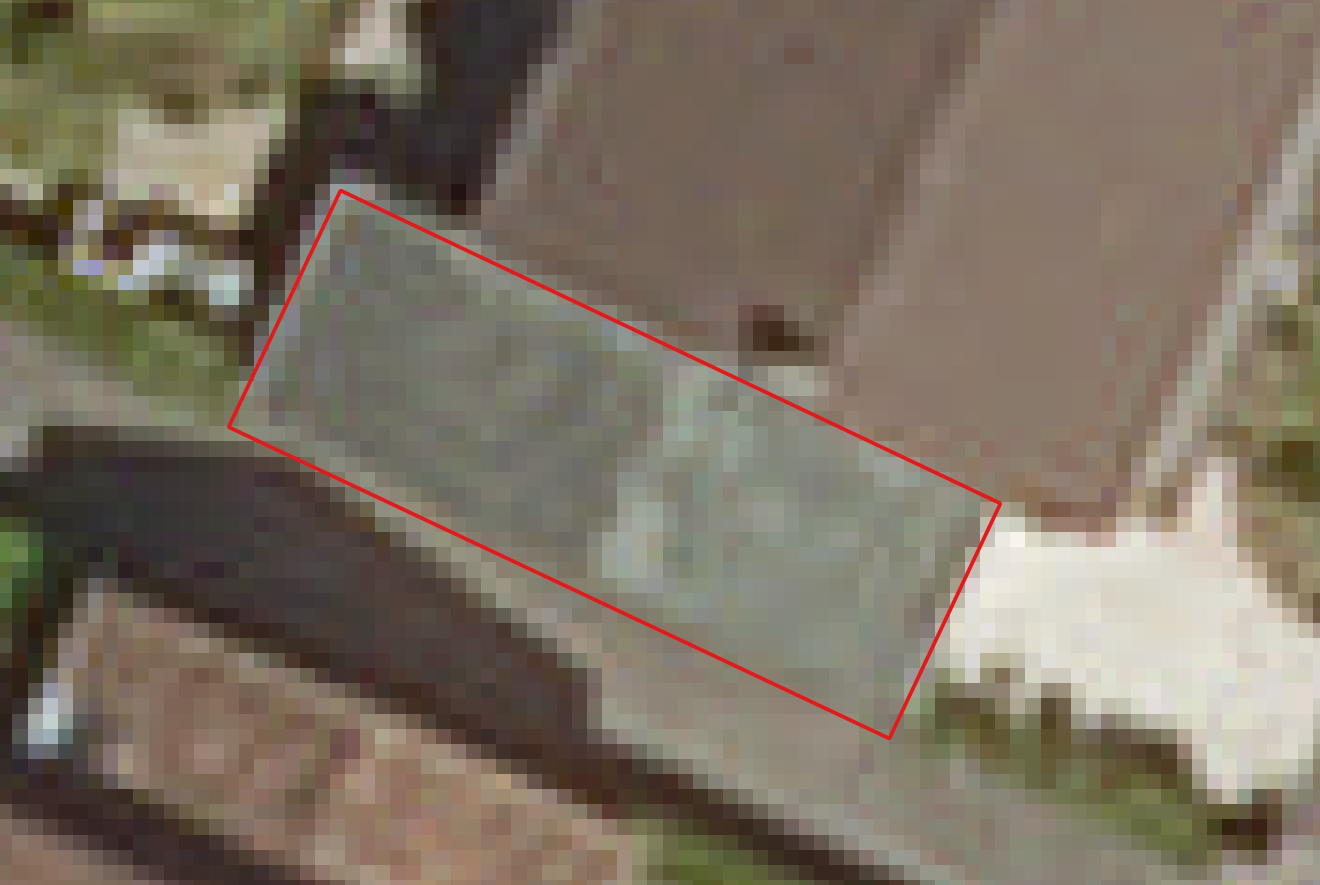
\includegraphics[width=.24\textwidth]{images/Facet_Errors/under_segmentation}}}
                        \ffigbox[\FBwidth]{\caption{Over segmentation.}\label{fig::over_fac}}{\fbox{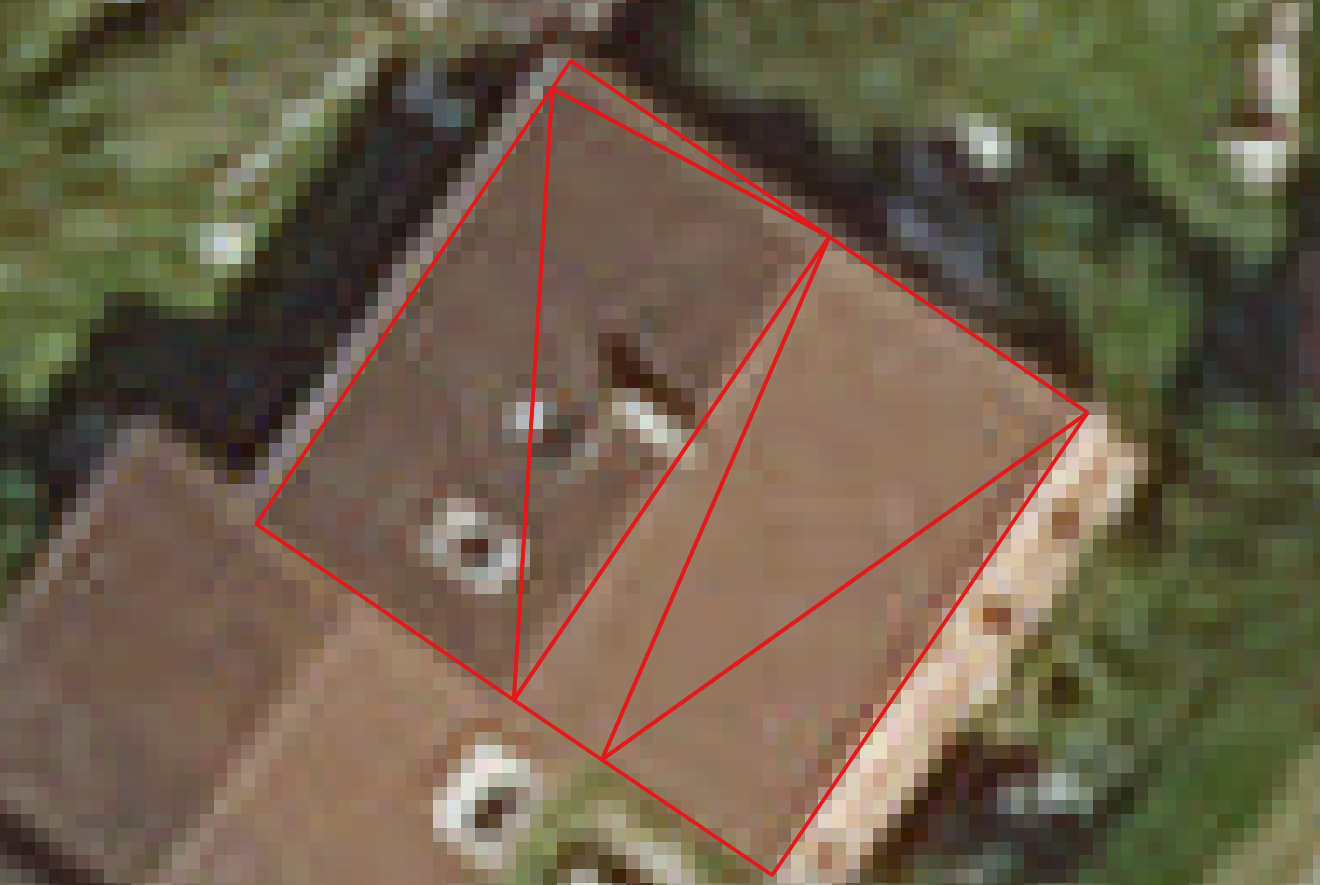
\includegraphics[width=.24\textwidth]{images/Facet_Errors/over_segmentation}}}
                        \ffigbox[\FBwidth]{\caption{Mis Segmentation.}\label{fig::mis}}{\fbox{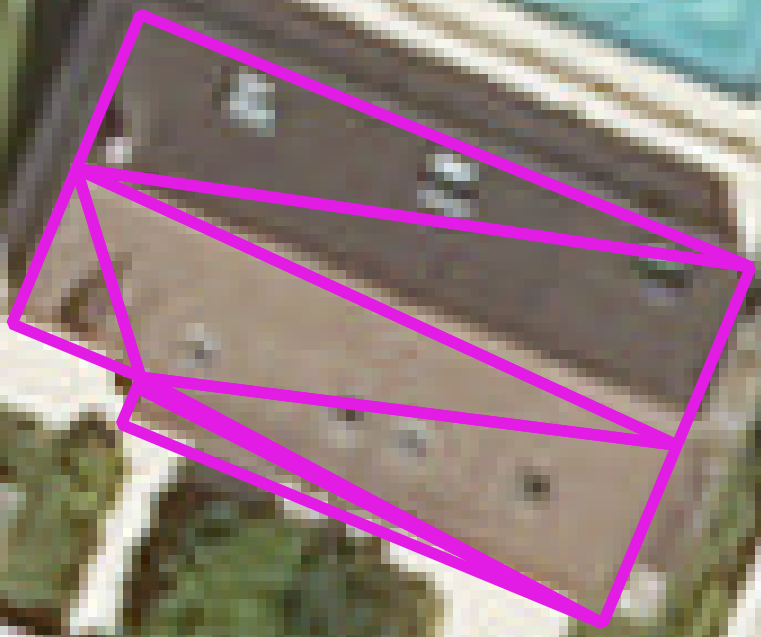
\includegraphics[width=.24\textwidth]{images/Facet_Errors/mis_segmentation}}}
                        \ffigbox[\FBwidth]{\caption{Imprecise slope.}\label{fig::slope}}{\fbox{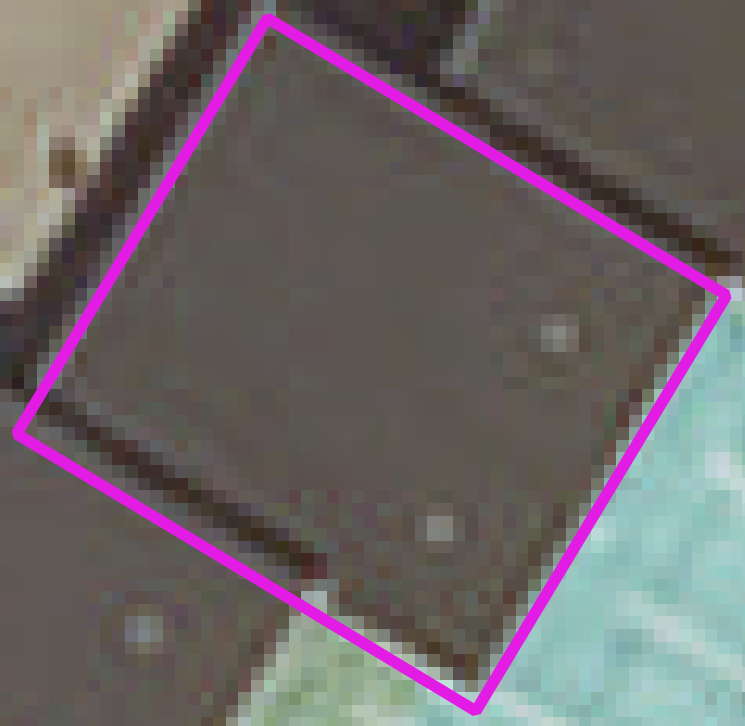
\includegraphics[width=.24\textwidth]{images/Facet_Errors/slope}}}
                    \end{subfloatrow}
                }
                {
                    \renewcommand\figurename{}
                    \renewcommand{\thefigure}{(\roman{SubFigCounter})}

                    \caption{Facet errors family samples.}\label{fig::fac_err}
                    \refstepcounter{SubFigCounter}
                }
            }
            {
                \addtocounter{figure}{-3}
                \caption{\label{fig::samples}Error samples illustrated.}
            }
        \end{center}
    \end{figure}
\subsection{Baseline Features}
\subsection{Classifiers}
\section{Experiments}
\subsection{Data}
\subsection{Results}
\subsection{Discussion}
\section{Conclusion}

\bibliographystyle{splncs}
\bibliography{references}
\end{document}
